\documentclass[landscape]{article}

%\usepackage[top=0.4in,bottom=0.4in,left=0.75in,right=0.5in]{geometry}
\usepackage[paperwidth=13.13636in,paperheight=8.5in,top=0.4in,bottom=0.3in,left=0.75in,right=0.75in]{geometry}  % aspect ratio same as 11x17 (1.5454)
\usepackage{graphicx}
\usepackage{caption}
\usepackage{subcaption}
\usepackage{nopageno}
\pagestyle{plain}
\usepackage{array}
\usepackage[export]{adjustbox}
\usepackage{tabularx} % table features
\usepackage{booktabs} % table features
\usepackage[abs]{overpic} % overlaying one graphic on another
\usepackage{xstring,xifthen} % string length with conditionals
\usepackage{color} % colored text
\usepackage{helvet} % font
%\usepackage{cmbright} % font
%\usepackage{avant} % font

\DeclareGraphicsExtensions{.pdf}

\renewcommand{\familydefault}{\sfdefault}

\parindent=0pt
\baselineskip=0pt
\parskip=0pt

% Barcode
\def\barcode{000005066}


% Sample Date
\def\sampledate{May 26, 2013}
\def\sampletime{1:40 pm}


% Abundance Table
\def\abundTaxonA{Genus \textit{Leuconostoc}}
\def\abundSamplA{23.4}

\def\abundTaxonB{Genus \textit{Staphylococcus}}
\def\abundSamplB{15.7}

\def\abundTaxonC{Genus \textit{Corynebacterium}}
\def\abundSamplC{11.7}

\def\abundTaxonD{Genus \textit{Lactobacillus}}
\def\abundSamplD{9.9}

\def\abundTaxonE{Genus \textit{Dermacoccus}}
\def\abundSamplE{8.6}



% Enrichment Table
\def\enrichTaxonA{Genus \textit{Vagococcus}}
\def\enrichSamplA{2.60}
\def\enrichPopulA{0.07}
\def\enrichFoldA{36}

\def\enrichTaxonB{Genus \textit{Leuconostoc}}
\def\enrichSamplB{23.40}
\def\enrichPopulB{0.78}
\def\enrichFoldB{30}

\def\enrichTaxonC{Genus \textit{Dermacoccus}}
\def\enrichSamplC{8.60}
\def\enrichPopulC{0.20}
\def\enrichFoldC{42}

\def\enrichTaxonD{Genus \textit{Rhodoplanes}}
\def\enrichSamplD{0.20}
\def\enrichPopulD{0.02}
\def\enrichFoldD{12}

\def\enrichTaxonE{Order Lactobacillales}
\def\enrichSamplE{0.60}
\def\enrichPopulE{0.08}
\def\enrichFoldE{8}



% Rare List
\def\rareList{Your sample contained the following rare  and \textcolor{red}{1 unique} taxa: \textcolor{red}{Genus \textit{Rathayibacter}}, Genus \textit{Carnobacterium}, Genus \textit{Rickettsiella}, Genus \textit{Marinomonas}.}



% Name
\def\yourname{Daley O'Earnhardt Jr. Jr.}



% Sample Type
\def\sampletype{skin}


%%%%%%%%%% BEGIN DOCUMENT / HEADER %%%%%%%%%%

\begin{document}

%\begin{tabularx}{\textwidth}{ X c X }     %<--does better with horizontal spacing
\begin{tabular}{ m{4.4cm} m{16cm} }  %<--does better with vertical spacing
	~~
\includegraphics[height=0.08\textheight]{pdfs-oralskin/logoshape.pdf} & 
\includegraphics[height=0.065\textheight]{pdfs-oralskin/youramericangutsampletext.pdf} \\
\end{tabular}

\hrule

\vspace{0.65cm}

%%%%%%%%%% NAME %%%%%%%%%%

\begin{center}

\StrLen{\yourname}[\yournameLen]

\ifthenelse{\yournameLen < 28}{
	{\fontfamily{phv}\fontsize{38}{48}\selectfont {\MakeUppercase {\bf \yourname}}}
}{
	{\fontfamily{phv}\fontsize{34}{46}\selectfont {\MakeUppercase {\bf \yourname}}}
}

\end{center}

\vspace{0.65cm}

%%%%%%%%%% FIRST ROW %%%%%%%%%%

{\huge What's in your \sampletype{} sample?}

\vspace{2mm}

\begin{tabular*}{\textwidth}{ m{0.3in} m{4.0in} m{7.5in} }
	&
	\vspace{2mm}
	\hspace{-5mm}
	\includegraphics[scale=0.27]{pdfs-oralskin/piechart.pdf}
	
    &
    {\normalsize 
    \vspace{2.5mm}
    \parbox[b][][t]{6.5in}{
	\begin{tabular}{ c l r c l r r r }
    \multicolumn{3}{l}{\large ~~Your most abundant microbes:} & \multicolumn{5}{l}{\large ~~Your most enriched microbes:}\\ \addlinespace[2mm]
        \cline{2-3} \cline{5-8} \addlinespace[1mm]
        & Taxonomy & Sample & & Taxonomy & Sample & Population & Fold \\
        \cline{2-3} \cline{5-8} \addlinespace[1mm]
        & \abundTaxonA{} & \abundSamplA{}\% & & \enrichTaxonA{} & \enrichSamplA{}\% & \enrichPopulA{}\% & \enrichFolddA{}x \\
        & \abundTaxonB{} & \abundSamplB{}\% & & \enrichTaxonB{} & \enrichSamplB{}\% & \enrichPopulB{}\% & \enrichFolddB{}x \\
        & \abundTaxonC{} & \abundSamplC{}\% & & \enrichTaxonC{} & \enrichSamplC{}\% & \enrichPopulC{}\% & \enrichFolddC{}x \\
        & \abundTaxonD{} & \abundSamplD{}\% & & \enrichTaxonD{} & \enrichSamplD{}\% & \enrichPopulD{}\% & \enrichFolddD{}x \\
        \cline{2-3} \cline{5-8} \addlinespace[3mm]
        & \multicolumn{7}{p{5.6in}}{\footnotesize \rareList{}} \\
        & \multicolumn{7}{p{5.6in}}{\footnotesize This sample was registered on \sampledate{} at \sampletime{}.}
	\end{tabular}
	}
	}
\end{tabular*}

\vspace{5mm}

%%%%%%%%%% SECOND ROW %%%%%%%%%%

{\huge How do your \sampletype{} microbes compare to others?} 

\vspace{-5mm}

\begin{tabular*}{\textwidth}{ m{0.3in} m{3.5in} m{3.7in} m{3.7in} }

&

\begin{overpic}[width=2.10in]{pdfs-oralskin/barchart.pdf}
	\ifthenelse{\equal{\sampletype}{oral}}{\put(-32,-42){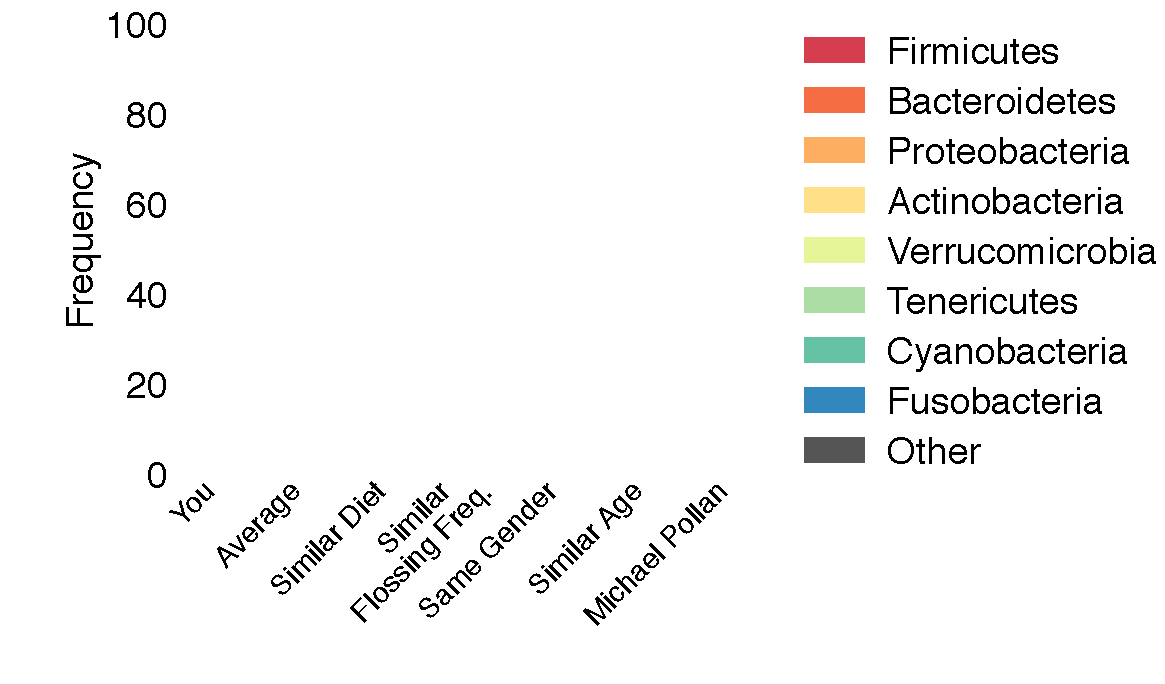
\includegraphics[width=3.65in]{pdfs-oralskin/barchart_overlay_oral.pdf}}}{}
	\ifthenelse{\equal{\sampletype}{skin}}{\put(-32,-42){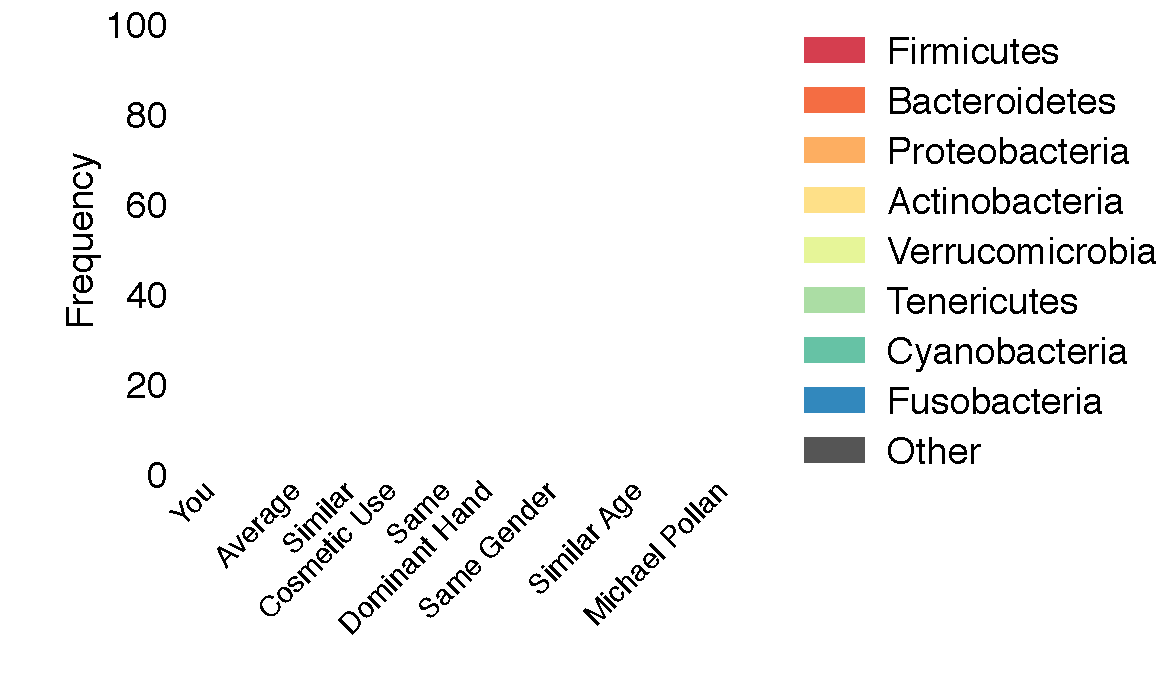
\includegraphics[width=3.65in]{pdfs-oralskin/barchart_overlay_skin.pdf}}}{}
\end{overpic} 

&

\vspace{10mm}
%\raisebox{29mm}{\includegraphics[scale=0.40]{pdfs-oralskin/hmppcoa_legend.pdf}}
\hspace{10mm}
\begin{overpic}[height=0.30\textheight]{pdfs-oralskin/hmppcoa.pdf}
	\put(0,-3){\includegraphics[scale=0.43]{pdfs-oralskin/hmppcoa_ovals.png}}
 	\put(130,185){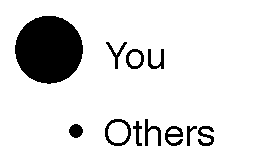
\includegraphics[scale=0.45]{pdfs-oralskin/ball_legend.pdf}}
 	\put(170,82){\includegraphics[scale=0.40]{pdfs-oralskin/hmppcoa_legend.pdf}}
\end{overpic}

&

\vspace{1cm}
\hspace{19mm}
\begin{overpic}[height=0.30\textheight]{pdfs-oralskin/agppcoa.pdf}
	\ifthenelse{\equal{\sampletype}{oral}}{\put(185,0){\includegraphics[scale=0.40]{pdfs-oralskin/agppcoa_legend_oral.pdf}}}{}
	\ifthenelse{\equal{\sampletype}{skin}}{\put(185,0){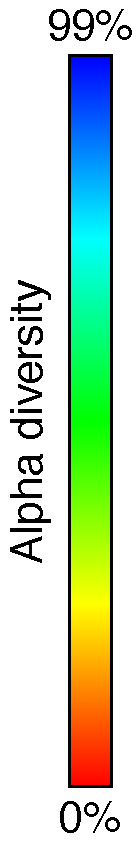
\includegraphics[scale=0.40]{pdfs-oralskin/agppcoa_legend_skin.pdf}}}{}
\end{overpic} 


\\ \addlinespace[-2mm]

% captions - change makebox to framebox to see borders of captions

& 

\hspace{9mm} \makebox[2in][c]{Different subpopulations} \par 

& 

\hspace{20mm} \makebox[2in][c]{Different body sites} \par 

& 

\hspace{30mm} \makebox[2in][c]{The American Gut population} \par

\end{tabular*}



\end{document}
